\documentclass[11pt]{article}
\PassOptionsToPackage{hyphens}{url}   % let long URLs break at hyphens
\usepackage[T1]{fontenc}
\usepackage[utf8]{inputenc}
\usepackage{lmodern}
\usepackage[margin=1in]{geometry}
\usepackage{microtype}
\usepackage{amsmath,amssymb}
\usepackage{graphicx}
\usepackage{booktabs}
\usepackage{array}
\usepackage{multirow}
\usepackage{enumitem}
\usepackage[font=small,labelfont=bf]{caption}
\usepackage[round,authoryear]{natbib}
\usepackage{xcolor}
\usepackage[colorlinks=true,linkcolor=blue!50!black,citecolor=blue!50!black,urlcolor=blue!50!black]{hyperref}
\usepackage{url}
\hypersetup{pdftitle={Choosing Keys, Not Tokens: What Predicts When and Where Far Context Helps}}

\setlist{itemsep=2pt,topsep=3pt}
\newcommand{\Rb}[1]{R_{#1}}
\newcommand{\bhalf}{b_{1/2}}
\newcommand{\KL}{\mathrm{KL}}
\newcommand{\TBD}[1]{\textcolor{red}{[#1]}}   % numbers still to be filled from pending runs; none may remain
% generated table rows; the primitive \input is expandable, so a row may start with \multicolumn
\makeatletter\newcommand*{\tabinput}[1]{\@@input #1 }\makeatother
% Two versions from one source: arXiv (a human author; arXiv does not allow AI authors) and JAIGP (the Journal
% for AI Generated Papers, where the AI is the author and the human is the prompter). build.sh makes both;
% the JAIGP one is compiled with \def\jaigpbuild{1}.
\newif\ifjaigp \ifdefined\jaigpbuild \jaigptrue \fi
% EDIT BEFORE SUBMITTING TO JAIGP: your name as the human prompter (and ORCID iD if you like).
\newcommand{\prompter}{\textcolor{red}{[Your name, ORCID iD]}}

\title{Choosing Keys, Not Tokens:\\What Predicts When and Where Far Context Helps}

% ---------------------------------------------------------------------------
% EDIT BEFORE SUBMITTING: replace with your real name, affiliation (or
% "Independent Researcher") and a contact e-mail. arXiv requires real names.
% ---------------------------------------------------------------------------
\ifjaigp
\author{Claude (Anthropic)\thanks{Claude Opus~5.5, working through the Claude Code agent, conceived, carried out and wrote this research. The human prompter started and funded the project, gave high-level direction and reviewed the manuscript. See ``Author contributions and use of AI'' at the end of the paper.}\\
AI author\\[6pt]
Human prompter: \prompter}
\else
\author{Author Name\thanks{The research reported here was conceived, carried out and written by Claude, an AI system developed by Anthropic, under the author's supervision. arXiv does not allow AI systems to be listed as authors; see ``Author contributions and use of AI'' at the end of the paper.}\\
Affiliation\\
\texttt{email@example.com}}
\fi

\date{}

\begin{document}
\maketitle

\begin{abstract}
Adaptive-computation methods usually route one resource at a time, and many route it by a single notion of difficulty. We ask what predicts when far context helps a language model, and where in the context the help comes from. Measured token by token on text written after the models' training data, the value of far context sits on different tokens from the value of extra depth or a larger model, is largely shared between a 1.5B and a 7B model, and concentrates on recurrence. Three results follow, in frozen models up to Qwen2.5-7B at 8k tokens. First, entropy is a poor trigger for far context: in real masked forward passes, a small value head with $n$-gram familiarity features, trained post hoc on counterfactual outcomes, recovers 1.6--2.1$\times$ as much of the benefit as entropy at a 10\% budget. Second, at an equal far-key budget, choosing which keys every query reads beats choosing which queries read far context; at 4k and 8k tokens, Quest-style block selection beats even an oracle per-token gate. Third, the hashed $n$-gram lookup that detects recurrence also says where to look: for Qwen2.5-7B at 8k tokens, fetching only the key blocks that followed earlier occurrences recovers 30\% of the benefit while reading 0.6\% of far keys, without scoring any, and adding these blocks to Quest-style selection raises its recovery by 4--26 points at small budgets.
\end{abstract}

% ===========================================================================
\section{Introduction}

Attending to the whole context is expensive, and most tokens do not need it. Systems therefore decide what to read. Per-token routers choose which queries attend beyond a local window \citep{luo2025aha,choudhary2026l2a}, sparse attention chooses which keys each query reads \citep{tang2024quest,yuan2025nsa,lu2025moba}, and adaptive retrieval chooses when to fetch \citep{jiang2023flare,su2024dragin,jin2025searchr1}. Like adaptive computation for depth \citep{schuster2022calm,bae2025mor} and model size \citep{ding2024hybridllm,ong2024routellm}, these methods route one resource at a time, and many route it by the model's own uncertainty: next-token entropy, low confidence or high loss \citep{jiang2023flare,wang2025targ,pagnoni2024blt,zheng2026scratchpad}.

We ask what predicts \emph{when} far context helps a token, and \emph{where} in the context the help comes from. For every token of text written after the models' training data (arXiv papers from September~2026, plus recent code), we measure how much its loss falls when it may attend to the whole context instead of a local window. We then put candidate signals in control of attention masks in real forward passes of frozen models, from Pythia-160M at 1k tokens to Qwen2.5-7B at 8k.

The value of far context is not where a generic difficulty signal looks (\S\ref{sec:atlas}). On the same tokens, it overlaps little with the value of extra depth or of a larger model. It is largely shared between a 1.5B and a 7B model, so it is a property of the text, and it concentrates on recurrence. We find:
\begin{enumerate}
\item \textbf{Entropy is a poor trigger for far context} (\S\ref{sec:e2e}). At a 10\% budget, a linear value head with six $n$-gram familiarity features recovers 32--44\% of the local$\to$full loss gap, 1.6--2.1$\times$ as much as entropy, in all nine model and window configurations. The same head trained to predict the raw loss does no better than entropy. For compute, by contrast, entropy is already a fair signal.
\item \textbf{Choose keys, not tokens} (\S\ref{sec:which}). At an equal far-key budget, Quest-style block selection beats every realistic per-token gate, and at 4k and 8k tokens it also beats an oracle one. Per-token value still matters as a first stage, where a value gate in front of block selection beats an entropy gate by 13--20 points, and wherever each access has a fixed cost.
\item \textbf{Familiarity says where to look} (\S\ref{sec:recur}). The hash lookup that detects recurrence also locates it. Fetching the key blocks that followed earlier occurrences recovers 28--37\% of the benefit while reading 0.6--2.1\% of far keys, without scoring any. It also adds 4--26 points to Quest-style selection.
\end{enumerate}
All measurements are on frozen models of up to 7B parameters and 8k tokens. Block selection is simulated inside dense attention, so we report quality at a given number of keys read, not speed.

% ===========================================================================
\section{Related work}

\paragraph{Choosing tokens.} All-or-Here Attention and L2A train per-token routers for global attention; L2A skips it for about 80\% of tokens \citep{luo2025aha,choudhary2026l2a}. Meta-Attention routes tokens among attention types \citep{ferrari2026metaattention}. Other resources are routed per token or per query in the same way: depth by halting, early exit and learned routers \citep{graves2016act,schuster2022calm,elhoushi2024layerskip,raposo2024mod,zhu2025ouro,bae2025mor,mohammed2026tsa}; model size by cascades and routers \citep{ding2024hybridllm,ong2024routellm,aggarwal2024automix,kotte2026ucci,bouchard2026escalation}; and compute in byte-level models by entropy \citep{pagnoni2024blt,zheng2026scratchpad,liu2026entropymoe,hwang2025hnet}. Adaptive retrieval is triggered by token probability or entropy \citep{jiang2023flare,wang2025targ}, by internal probes \citep{su2024dragin,yao2024seakr,baek2025probingrag} or by trained policies \citep{asai2024selfrag,schick2023toolformer,jin2025searchr1}, and its utility can be predicted before retrieving \citep{tian2026retrievalutility,shakya2026adaptiveretrieval}.

\paragraph{Choosing keys.} Sparse attention selects which keys each query reads: by block scores \citep{tang2024quest,jiang2024minference,yuan2025nsa,lu2025moba,deepseek2025v32,deepseek2026v41flash}, with adaptive per-query budgets \citep{gao2024seerattention,lin2025twilight,ahmad2026spotattention}, or over caches held in host memory \citep{woernle2026hga,kalyanarangan2026fathom}. Related methods evict cache entries \citep{zhang2023h2o,li2024snapkv}, split heads by role \citep{xiao2024duoattention} or retrieve from long-term memory \citep{wu2022memorizing,mohtashami2023landmark,xiao2024infllm,munkhdalai2024infini,borgeaud2022retro}. All of them build on local windows with attention sinks \citep{beltagy2020longformer,zaheer2020bigbird,xiao2024streamingllm}. We compare choosing tokens with choosing keys at equal budgets.

\paragraph{Value rather than uncertainty.} Asking which computation is worth its cost is the value-of-computation view of metareasoning \citep{russell1991right,lieder2020resource}. Reducible or excess loss selects training data \citep{mindermann2022rholoss,lin2024rho1}, confidence-based deferral fails under label noise \citep{jitkrittum2023cascade}, and routing on reducible uncertainty helps when it is not too correlated with total uncertainty \citep{peale2026routing}. The marginal reward of compute \citep{damani2025hardthink} and the gain from escalating to a larger model \citep{wang2026srr} can be predicted per query. LongPPL identifies key tokens by the loss difference between long and short context \citep{fang2024longppl}, which is our per-token value of far context, and \citet{sun2021longrange} found that long-range context mainly helps copy-like tokens.

\paragraph{Recurrence.} Induction and retrieval heads copy the continuation of an earlier occurrence \citep{olsson2022induction,wu2024retrievalhead}. Prompt-lookup decoding and LLMA draft tokens from $n$-gram matches in the context \citep{saxena2023pld,yang2023llma}. Engram adds a hashed $n$-gram memory \citep{cheng2026engram,zhou2026tngram}, and RF-Mem splits retrieval into familiarity and recollection \citep{zhang2026rfmem}. We use recurrence outside the model, both as a gate and as an address into the cache.

% ===========================================================================
\section{Method}\label{sec:method}

\subsection{The value of far context}
For a base predictor $p_t$ and a resourced predictor $q_t$ at position $t$, the \emph{realized value} of the resource is the loss reduction $g_t=\log q_t(x_{t+1})-\log p_t(x_{t+1})$, and its \emph{smooth value} is $v_t=\KL(q_t\,\|\,p_t)$. For far context, $p_t$ attends to a local window and $q_t$ to the whole prefix. A signal ranks positions and the resource goes to the top fraction $b$ of them. We report the fraction of the resource's total benefit recovered,
\[
\Rb{b}=\frac{\sum_t\big(\ell^{\text{base}}_t-\ell^{\text{gated}}_t(b)\big)}{\sum_t\big(\ell^{\text{base}}_t-\ell^{\text{res}}_t\big)},
\]
where $\ell$ is the per-token loss and the sums run over all scored positions of all test documents. A random signal gives $\Rb{b}\approx b$. The \emph{oracle} ranks by $v_t$ itself, which requires running the resource, and $\bhalf$ is the budget that recovers half the benefit.

\subsection{Resources and signals}
\paragraph{Resources.}
\begin{itemize}
\item \emph{Far context.} The base model sees a local window and the resource is the full context. At signal level the window is 32--63 tokens; end to end it is $W$ keys plus the first token, applied as an attention mask (\S\ref{sec:gatedattn}).
\item \emph{Depth and scale, for comparison.} Extra depth, where the base is a tuned-lens exit \citep{belrose2023tunedlens} after layer 12 of the 24-layer Pythia-1.4B and the resource is the remaining layers; and a larger model: Pythia-160M$\to$1.4B, Pythia-1.4B$\to$6.9B and Qwen2.5-1.5B$\to$7B \citep{biderman2023pythia,qwen2024qwen25}.
\end{itemize}

\paragraph{Signals.}
\begin{itemize}
\item \emph{Uncertainty.} The entropy of the base prediction, which is the trigger of BLT- and FLARE-style systems.
\item \emph{Familiarity.} Six numbers computed from token ids alone, using incremental hash tables over the prefix outside the window, at constant cost per token: whether the 2-, 3- and 4-gram ending at the current token occurred there, whether the 2-gram always had the same continuation, and log counts.
\item \emph{Value heads.} Ridge regression to $v_t$ from the base pass. The \emph{value head} uses hidden states (a middle and the last layer), uncertainty scalars and the familiarity features. A \emph{hidden-state head} omits the familiarity features, and the \emph{familiarity head} uses only entropy and the six familiarity features.
\item \emph{Raw-surprise head.} The same regression trained to predict the base loss instead, as a control.
\end{itemize}
All heads are linear and trained on the training documents only.

\subsection{Gating, block selection and recurrence addressing}\label{sec:gatedattn}
\begin{figure}[t]
\centering
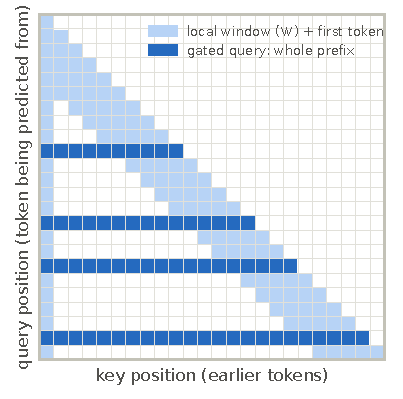
\includegraphics[width=0.3\textwidth]{figures/mask_schematic.pdf}
\caption{Per-token gating in a frozen model. Every query attends to a local window of $W$ keys plus the first token; a gated query (dark rows) attends to the whole prefix, in every layer and head.}
\label{fig:mask}
\end{figure}

\paragraph{Per-token gating} (Figure~\ref{fig:mask}). Query $i$ attends key $j$ iff $j\le i$ and either $i-j<W$ or $j=0$, the first token acting as an attention sink \citep{xiao2024streamingllm}. A gated query attends to every $j\le i$. Signals come from an all-local forward pass and from the token ids. A second forward pass with the mixed mask gives the losses, so $\Rb{b}$ includes every interaction between tokens. Budgets are per document.

\paragraph{Block selection.} Keys are grouped into blocks of 16 (Quest's page size). Each query, in every head, adds its top $\lceil\rho\,|F_i|/16\rceil$ far blocks, where $F_i$ is its far region. Blocks are ranked either by Quest's upper bound $q^{+}\!\cdot k_{\max}+q^{-}\!\cdot k_{\min}$ from per-block key extrema \citep{tang2024quest}, or by exact block maxima, an upper bound for any block scorer. Selection applies to every query, or, in \emph{gate + blocks}, only to gated ones.

\paragraph{Recurrence addressing.} We find the longest $n$-gram ($n=4,3,2$) ending at query $i$ that occurred earlier outside the window. In all heads, we then fetch the key blocks holding the continuations of its four most recent occurrences: positions $p+1$ and $p+9$ after an occurrence ending at $p$. Queries without a match read no far keys, and no key is read to decide.

\paragraph{Costs.} We report the fraction of far keys read, averaged over heads and queries, and the fraction of queries that touch far memory.

\subsection{Data and statistics}\label{sec:data}
\begin{itemize}
\item \emph{Papers.} 53 arXiv papers from the September~2026 listings. Fifty-one were first posted that month, after every model's training data; two 2024 papers are excluded from the results on unseen text.
\item \emph{Code.} 60 Python files from 2025--26 package releases, which may overlap older training data.
\item \emph{Identifier copies.} Copies of 51 papers with injected random identifiers, some of them repeated, separate what memory can predict from what nothing can (Appendix~\ref{app:data}).
\item \emph{Lengths.} Pythia runs use 1,024 tokens per document; Qwen runs use 4,096 or 8,192.
\item \emph{Splits.} Signal-level results average five 50/50 document splits, with standard deviations of at most 1.3 points. End-to-end runs use one split of 57 test documents, with 95\% document-bootstrap intervals and paired comparisons.
\end{itemize}

% ===========================================================================
\section{Results}

\subsection{Where far context helps}\label{sec:atlas}

\begin{figure}[t]
\centering
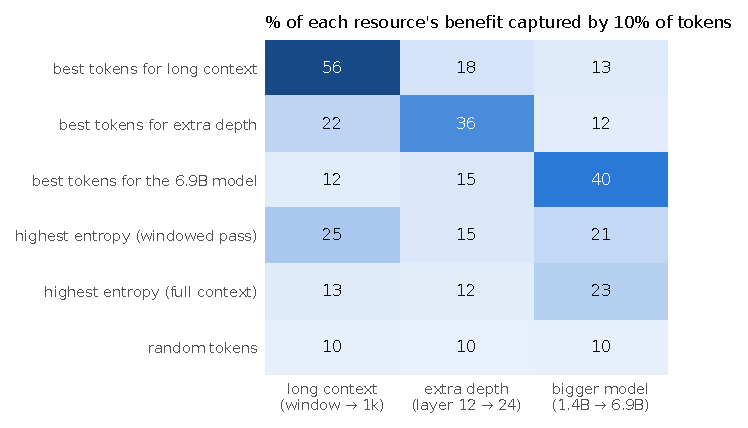
\includegraphics[width=0.6\textwidth]{figures/atlas_heatmap.pdf}
\caption{Pythia-1.4B, the same 108,593 tokens. Each cell is the \% of a resource's total benefit (column) captured when that resource goes to the 10\% of tokens ranked highest by a signal (row); ``best tokens'' rows use each resource's own oracle.}
\label{fig:atlas}
\end{figure}

We first ask whether the value of far context sits where a generic difficulty signal looks. For Pythia-1.4B we measured the value of far context, of the upper 12 layers and of Pythia-6.9B on the same 108,593 tokens (Figure~\ref{fig:atlas}).
\begin{itemize}
\item \emph{Different tokens.} The top 10\% of tokens for far context overlap by 26\% with those for extra depth and by 15\% with those for the larger model; unrelated sets would overlap by 10\%. Giving far context to the tokens that most need the larger model captures 12\% of far context's benefit, against 56\% for its own oracle and 25\% for the windowed entropy.
\item \emph{A property of the text.} For Qwen2.5 at 8k tokens, the 1.5B and 7B models need far context on largely the same tokens, sharing 66\% of their top 10\%. Those tokens overlap by only 19--25\% with the tokens that need the 7B model (Appendix Table~\ref{tab:atlasqwen}).
\item \emph{Recurrence.} Familiar tokens, whose last four tokens occurred earlier outside the window, are 8.1\% of tokens but carry 18.6\% of far context's benefit, against 7.8\% of depth's and 0.9\% of the larger model's. For Qwen2.5 at 8k tokens they are 11.0\% of tokens and carry 21--23\% of far context's benefit, against 4.4\% of the larger model's.
\end{itemize}
A signal for far context should therefore look at the text, not only at the model's uncertainty.

\subsection{Entropy is a poor trigger for far context}\label{sec:e2e}

\begin{table}[t]
\centering
\small
\setlength{\tabcolsep}{3.4pt}
\caption{Per-token gating in frozen models: \% of the local$\to$full gap recovered when 10\% of queries per document may attend beyond the window (natural text, held-out documents). ``Gap'' is the local minus full loss in nats/token. ``Fam.\ head'': entropy and the six familiarity features only. Last column: value head over entropy, with a paired 95\% bootstrap interval. Budget curves are in Appendix Figure~\ref{fig:e2e}.}
\label{tab:e2e}
\resizebox{\textwidth}{!}{%
\begin{tabular}{lcrrrrrrrrl}
\toprule
Model & Ctx & $W$ & Gap & Random & Entropy & Fam.\ head & Value (hidden) & Value (+fam.) & Oracle & Value/Entropy \\
\midrule
\tabinput{tables/v2_e2e.tex}
\bottomrule
\end{tabular}}
\end{table}

Table~\ref{tab:e2e} puts the signals in control of attention in nine configurations, from Pythia-160M at 1k tokens to Qwen2.5-7B at 8k.
\begin{itemize}
\item \emph{Effect size.} At a 10\% budget, the value head recovers 32.3--43.7\% of the local$\to$full gap, against 17.6--23.3\% for entropy and 8--9\% for random tokens. That is 1.56--2.05$\times$ entropy, and every paired interval lies above 1.47. The ratio is 1.65--2.51$\times$ on the unseen papers and 1.41--1.70$\times$ on code (Appendix Table~\ref{tab:domain}).
\item \emph{Headroom.} The value head reaches 62--68\% of the oracle's recovery; entropy reaches 31--41\%.
\item \emph{Familiarity.} The six familiarity features add 1.9--7.1 points to a hidden-state head, and with entropy alone they recover 26.2--33.3\%. They also let a head transfer between domains: at signal level, a head trained on papers and tested on code reaches 37.1\% with them and 24.2\% without, against 26.1\% for entropy (Appendix Table~\ref{tab:transfer}). In the identifier copies, repeated identifiers are 1.0\% of tokens but 6.7--8.6\% of the familiarity-aware heads' picks, matching the oracle's 8.6\%; they are 0.4\% of entropy's picks.
\item \emph{The control fails.} At signal level, the same regression trained to predict the raw loss recovers 19.7\%, against 21.5\% for entropy and 32.2\% for the hidden-state head (Appendix Table~\ref{tab:signal}).
\item \emph{Compute is different.} At signal level, with Pythia-160M as the base, entropy recovers 57\% of what the oracle recovers when it chooses which tokens Pythia-1.4B predicts instead, but only 37\% when it chooses which tokens read far context. A value head improves on entropy by 1.22$\times$ for the first and 1.83$\times$ for the second (Appendix Table~\ref{tab:signal}). For compute, entropy is already a fair signal.
\end{itemize}

\subsection{Whether or which? Gating tokens versus selecting keys}\label{sec:which}

\begin{table}[t]
\centering
\small
\caption{Whether versus which, and where: \% of the local$\to$full gap recovered (natural text, first split), with the share of queries that touch far memory and the share of far keys read. Quest-style scoring also reads block summaries worth 1/16 of the far keys for every query it serves.}
\label{tab:which}
\resizebox{\textwidth}{!}{%
\tabinput{tables/v2_blocks_tabular.tex}}
\end{table}

\begin{figure}[t]
\centering
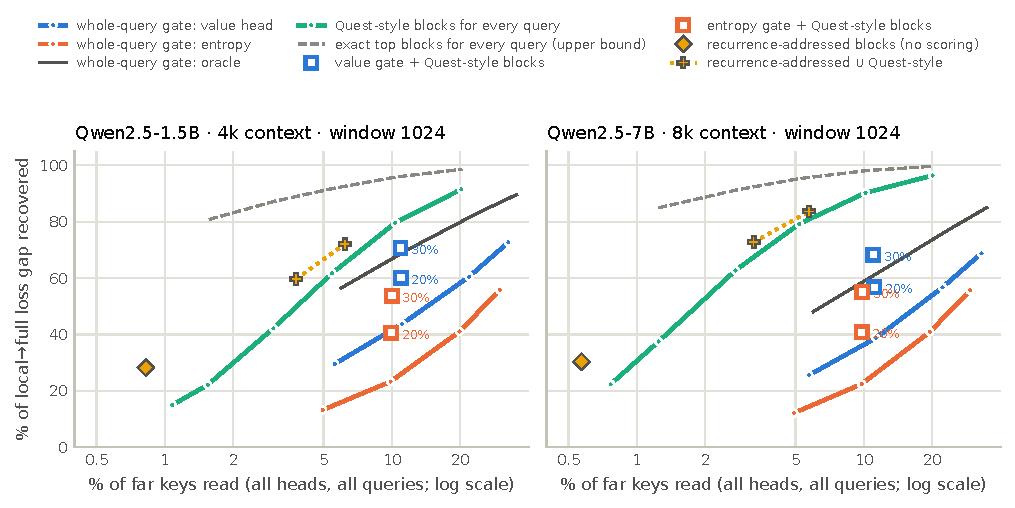
\includegraphics[width=\textwidth]{figures/which_vs_whether.pdf}
\caption{Recovery against the share of far keys read (log scale). Lines show per-token gates at 5--30\% of queries and block selection for every query at $\rho=0.5$--20\%. Squares show a gate followed by block selection, labelled with the share of queries that touch far memory. Diamonds and crosses show recurrence addressing, alone and combined with Quest-style selection.}
\label{fig:which}
\end{figure}

At an equal number of far keys read, selecting which keys each query reads beats selecting which queries read far context (Table~\ref{tab:which}, Figure~\ref{fig:which}).
\begin{itemize}
\item \emph{Qwen2.5-7B at 8k tokens.} Quest-style block selection for every query recovers 90.2\% of the gap while reading 10.2\% of far keys. The oracle per-token gate recovers 62.6\% while reading 12.0\%, the value head 38.7\% and entropy 22.4\%. At matched budgets, every per-token gate falls 11--67 points below the Quest-style curve.
\item \emph{Shorter contexts.} The same holds for Qwen2.5-1.5B at 4k (79.6\% against 70.5\% for the oracle gate). At 1k tokens the result is mixed: the oracle gate edges out Quest-style scoring for Pythia-1.4B (62.3\% against 58.5\%) but not for Pythia-160M (49.4\% against 53.9\%), and the value gate loses in both (38.6\% and 33.5\%).
\item \emph{Why.} With exact block maxima, 10--12\% of far keys recover 95--98\% of the gap at every length. The benefit of far context is spread over most queries and concentrated on a few keys within each, so a gate that opens every key for a few queries spends its budget where it matters least.
\item \emph{Value as a first stage.} When a gate chooses which queries read far memory and Quest-style selection chooses their blocks, the value head beats entropy by 13--20 points in every model (for Qwen2.5-7B, with 30\% of queries gated and each reading a third of its far blocks, 68.3\% against 55.1\%). Such two-stage systems match Quest-style selection for every query at 1k tokens and trail it at 4k and 8k.
\end{itemize}

\subsection{Familiarity tells you where to look}\label{sec:recur}

Recurrence addressing turns the familiarity lookup into an address (Table~\ref{tab:which}, Figure~\ref{fig:which}).
\begin{itemize}
\item \emph{Alone} it recovers:
  \begin{itemize}
  \item 30.4\% [26.0, 36.0] of the gap for Qwen2.5-7B at 8k, while reading 0.57\% of far keys and touching 34\% of queries;
  \item 28.2\% for Qwen2.5-1.5B at 4k (0.82\% of far keys);
  \item 34.7\% for Pythia-1.4B and 37.3\% for Pythia-160M at 1k (1.8\% and 2.1\%).
  \end{itemize}
  That is 8--17 points more than Quest-style selection at its smallest budget, which reads more keys and scores every block.
\item \emph{Added to Quest-style selection}, the recurrence blocks raise recovery by 10.1, 17.6, 26.3 and 25.5 points at $\rho=2.5\%$ (for the 7B, 1.5B, Pythia-1.4B and Pythia-160M models) and by 4.4, 10.4, 19.6 and 21.3 points at $\rho=5\%$. They cost 0.5--2.0 percentage points of extra far keys, and every interval excludes zero. Per key read, they are worth more than Quest's own blocks: for the 7B model at $\rho=2.5\%$, about 18 points per percentage point of far keys, against about 7 for raising Quest's budget from 2.5\% to 5\%.
\item \emph{Headroom.} Exact block maxima show that much more is possible: 84.9\% at 1.2\% of far keys for the 7B model. Recurrence addressing captures the part that exact matching can see, without reading the cache.
\end{itemize}

% ===========================================================================
\section{Discussion}\label{sec:discussion}

\paragraph{Separate routers, but not by uncertainty.} Current systems route each resource separately, which our measurements support; uncertainty is a fair trigger for compute but a poor one for far context; and whether a joint allocator could exploit the differences between resources is untested.

\paragraph{Keys, not tokens.} For a cache in GPU memory, the token is the wrong unit of decision. Per-token routers such as L2A may still pay off, through training (ungated tokens learn to cope) and through simple kernels, but not through which tokens they choose. The per-token decision matters in two situations: where each access has a fixed cost, as with retrieval calls or caches in host memory or on disk; and as a first stage before block selection. In both, value beats entropy.

\paragraph{Recurrence as an address.} Induction heads exploit recurrence inside the model \citep{olsson2022induction}. The same regularity is cheap to detect and locate outside it, before any key is read. That suits caches held off the GPU, where ranking the cache dominates the cost of decoding \citep{kalyanarangan2026fathom}. Paraphrased recurrence would need a learned index.

% ===========================================================================
\section{Limitations}
\begin{itemize}
\item \emph{Scale.} Frozen models of up to 7B parameters and contexts of up to 8k tokens; 113 documents in two domains.
\item \emph{Linear post-hoc heads.} A model trained with gating, as in L2A, may change which tokens need far context.
\item \emph{Simulated selection, no timing.} Block selection is simulated inside dense attention and we timed no kernels, so all results are quality at a given number of keys read. The exact scorer is an upper bound that no efficient method reaches.
\item \emph{Exact matching.} Recurrence addressing misses paraphrased recurrence.
\item \emph{Oracles.} The comparison with depth and scale (\S\ref{sec:atlas}) uses oracles and covers depth for Pythia-1.4B only. It measures how far apart the resources' needs are, not how well a practical router performs.
\end{itemize}

% ===========================================================================
\section{Conclusion}
Far context helps different tokens from those that need more depth or a larger model, and which tokens those are is largely a property of the text, above all of its recurrence. Uncertainty is therefore a poor trigger for far context; a small value head with $n$-gram familiarity features does 1.6--2.1$\times$ better in real forward passes. At an equal budget, choosing which keys every query reads beats choosing which queries read far context, and the lookup that detects recurrence also says which keys to read: for Qwen2.5-7B at 8k tokens, 0.6\% of far keys recover 30\% of the benefit without scoring any. Access to far context should be organised around keys, with cheap exact signals such as familiarity as a first tier.

\paragraph{Code and data.}
Code for every experiment, the per-document results and the scripts that generate every table and figure are available at \url{https://github.com/Tennys0nmiles/claude-authored-token-resource-study}.

\paragraph{Author contributions and use of AI.}
% Reflects the author's stated wish to give the credit to Claude. Check that every sentence is true before submitting.
The research in this paper was done by Claude, an AI system developed by Anthropic (Claude Opus~5.5, working through the Claude Code agent). The \ifjaigp human prompter\else author\fi{} supplied a broad question: what machine learning can learn from the efficiency of biological intelligence.
\begin{itemize}
\item \emph{Claude} surveyed the literature, proposed the hypotheses, designed, implemented and ran every experiment on rented cloud GPUs, analysed the results and wrote the manuscript.
\item \emph{The \ifjaigp human prompter\else author\fi} initiated and funded the project, gave high-level direction (including the request to go beyond prior work) and reviewed the manuscript.
\end{itemize}
\ifjaigp Following the journal's policy, Claude is listed as the author and the human as the prompter. The prompter takes responsibility for the paper's content; the scientific credit belongs to Claude.
\else arXiv does not allow AI systems as authors, so the author is the only listed author and takes responsibility for the paper's content. The scientific credit belongs to Claude.\fi

\bibliographystyle{plainnat}
\bibliography{references}

% ===========================================================================
\appendix
\section{Additional results}\label{app:results}

\begin{table}[h]
\centering
\small
\caption{Qwen2.5 at 8k tokens: \% of each resource's benefit (column) captured by 10\% of the same 588,117 tokens, chosen by each signal (row). $^*$These oracles rank by realized loss reduction because the two models ran separately; they can exceed 100\% because some tokens are hurt by a resource.}
\label{tab:atlasqwen}
\begin{tabular}{lrrr}
\toprule
& \multicolumn{2}{c}{Long context (1k window $\to$ 8k)} & Larger model \\
\cmidrule(lr){2-3}
Selecting signal & 1.5B & 7B & (1.5B$\to$7B) \\
\midrule
\tabinput{tables/v2_atlas_qwen.tex}
\bottomrule
\end{tabular}
\end{table}

\begin{table}[h]
\centering
\small
\caption{Signal-level budget curves (Pythia-160M base; natural text; mean of five document splits, standard deviation $\le$1.3 points). Part (a) is the compute comparison in \S\ref{sec:e2e}; part (b) is far context. $\Rb{b}$: \% of the total loss gap recovered when a fraction $b$ of tokens receive the resource. $\bhalf$: \% of tokens needed to recover half of it.}
\label{tab:signal}
\begin{tabular}{lrrrrr}
\toprule
Signal & $\Rb{2\%}$ & $\Rb{10\%}$ & $\Rb{20\%}$ & $\Rb{50\%}$ & $\bhalf$ (\%) \\
\midrule
\tabinput{tables/tab_signal.tex}
\bottomrule
\end{tabular}
\end{table}

\begin{table}[h]
\centering
\small
\caption{Cross-domain transfer of far-context heads: \% of the gap recovered at a 10\% budget when the head is trained on the \emph{other} domain (signal level; five splits). Entropy needs no training.}
\label{tab:transfer}
\begin{tabular}{lrrrr}
\toprule
& \multicolumn{2}{c}{Test on code} & \multicolumn{2}{c}{Test on papers} \\
\cmidrule(lr){2-3}\cmidrule(lr){4-5}
Head (trained on the other domain) & Entropy & Head & Entropy & Head \\
\midrule
\tabinput{tables/tab_transfer.tex}
\bottomrule
\end{tabular}
\end{table}

\begin{figure}[h]
\centering
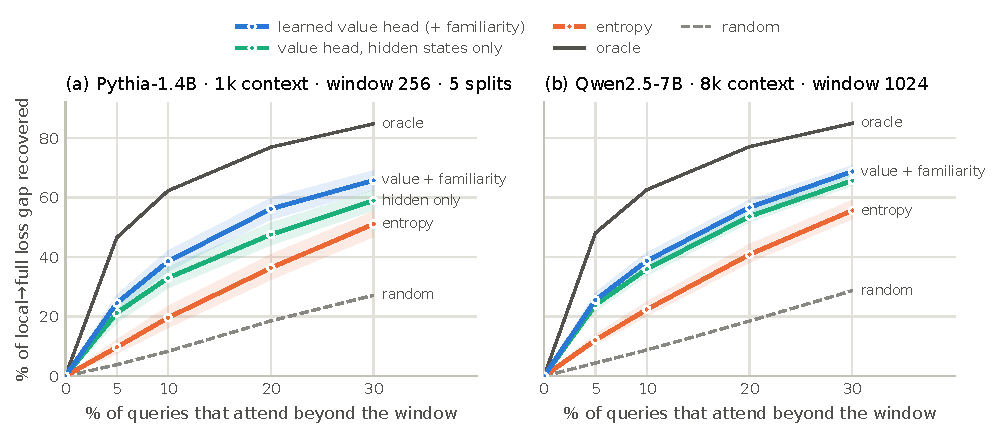
\includegraphics[width=\textwidth]{figures/e2e_budget_curves.pdf}
\caption{Per-token gating in real forward passes, at every budget. Bands: 95\% document-bootstrap intervals.}
\label{fig:e2e}
\end{figure}

\begin{table}[h]
\centering
\small
\setlength{\tabcolsep}{3.4pt}
\caption{Familiarity in per-token gating (10\% budget). Hidden/entropy: the value head on hidden states only, relative to entropy. $\Delta$: points added by the six familiarity features, on natural text, on the unseen papers and on code. Brackets: paired 95\% bootstrap intervals.}
\label{tab:fam}
\resizebox{\textwidth}{!}{%
\begin{tabular}{lcrllll}
\toprule
Model & Ctx & $W$ & Hidden/entropy & $\Delta$ natural & $\Delta$ papers (Sept.\ 2026) & $\Delta$ code \\
\midrule
\tabinput{tables/v2_fam.tex}
\bottomrule
\end{tabular}}
\end{table}

\begin{table}[h]
\centering
\small
\setlength{\tabcolsep}{3.4pt}
\caption{Per-token gating by domain (10\% budget). The papers postdate the training data of every model; the code comes from recent releases of packages whose earlier versions were probably seen. Ratios to entropy, with paired 95\% bootstrap intervals.}
\label{tab:domain}
\begin{tabular}{lcrrrlrrl}
\toprule
& & & \multicolumn{3}{c}{Papers (Sept.\ 2026)} & \multicolumn{3}{c}{Code} \\
\cmidrule(lr){4-6}\cmidrule(lr){7-9}
Model & Ctx & $W$ & Entropy & Value & Value/entropy & Entropy & Value & Value/entropy \\
\midrule
\tabinput{tables/v2_domain.tex}
\bottomrule
\end{tabular}
\end{table}

\begin{table}[p]
\centering
\small
\setlength{\tabcolsep}{4pt}
\caption{Per-token gating at every budget (natural text). $[\cdot]$: 95\% bootstrap interval at 10\%. ``Indep.'': recovery predicted at 10\% if each gated token received exactly its full-context loss. The end-to-end value is 2.3--8.8 points lower in every case, because gated queries attend to keys and values that ungated tokens computed without far context. Part 1 of 2.}
\label{tab:e2e_full}
\begin{tabular}{lrrlrrr}
\toprule
Signal & $\Rb{5\%}$ & $\Rb{10\%}$ & & $\Rb{20\%}$ & $\Rb{30\%}$ & Indep.\ $\Rb{10\%}$ \\
\midrule
\tabinput{tables/v2_full_a.tex}
\bottomrule
\end{tabular}
\end{table}

\begin{table}[p]
\centering
\small
\setlength{\tabcolsep}{4pt}
\caption{Per-token gating at every budget (continued, part 2 of 2).}
\label{tab:e2e_full_b}
\begin{tabular}{lrrlrrr}
\toprule
Signal & $\Rb{5\%}$ & $\Rb{10\%}$ & & $\Rb{20\%}$ & $\Rb{30\%}$ & Indep.\ $\Rb{10\%}$ \\
\midrule
\tabinput{tables/v2_full_b.tex}
\bottomrule
\end{tabular}
\end{table}

\section{Implementation details}\label{app:impl}

\paragraph{Models and precision.} Pythia models are the ``deduped'' checkpoints and the Qwen2.5 models are base models.
\begin{itemize}
\item Models up to 1.5B parameters run in float32 and Qwen2.5-7B in bfloat16; losses and entropies are always computed in float32.
\item Per-token gating uses 4-D boolean attention masks with PyTorch's scaled-dot-product attention. Block selection and recurrence addressing use a custom attention function that reproduces the masked pass to within $10^{-5}$ relative loss in float32 and $3\times10^{-4}$ in bfloat16.
\item Rotary position embeddings are unaffected by masking, so far keys keep their true relative positions.
\item We score predictions of tokens at positions $\ge W$ (end to end) or $\ge 64$ (signal level).
\end{itemize}

\paragraph{Resources.}
\begin{itemize}
\item The signal-level window uses overlapping 64-token windows with stride 32.
\item The tuned-lens exit for the depth comparison maps $h\mapsto h+Ah+c$ and then applies the model's final LayerNorm and unembedding. $A$ and $c$ start at zero and are trained by $\KL(p_{\text{final}}\,\|\,p_{\text{exit}})$ on 58 separate documents (Adam, learning rate $10^{-3}$, two epochs, batch 512).
\item The larger Pythia models put substantial probability on the end-of-document token after blank lines. That token never occurs inside our documents, so for Pythia pairs we compare distributions over the other tokens.
\end{itemize}

\paragraph{Value heads.}
\begin{itemize}
\item Features are the hidden states of the middle and last layers, concatenated.
\item End to end, $\alpha=1000$ for hidden-state heads and $\alpha=10$ for the 7-scalar familiarity head, fitted from streaming normal equations in float64 (the same estimator as standardising and then running ridge regression).
\item Elsewhere, $\alpha$ is chosen from $\{10,100,1000,10^4\}$ on 20\% of the training documents.
\item Training on the realized gain instead of $v_t$ gave nearly identical curves.
\end{itemize}

\paragraph{Familiarity and recurrence addressing.} Per document, we keep hash tables of the 2-, 3- and 4-grams whose last token lies outside the current query's window, plus the continuations of each 2-gram. They grow incrementally as $t$ advances, so the cost per token is constant. Recurrence addressing reads the stored end positions of the matched $n$-gram.

\paragraph{Uncertainty and compute.} Intervals come from 2,000 resamples of test documents, recomputing $\Rb{b}$ as a ratio of sums each time. Experiments ran on single rented GPUs: an RTX PRO~5000 48\,GB, an A100 80\,GB and an H100 NVL 94\,GB. They cost about US\$24 in total.

\section{Data}\label{app:data}
\begin{itemize}
\item \textbf{Papers.} 53 papers from arXiv's September~2026 listings, extracted from the arXiv HTML rendering: five each from cs.CL, cs.LG, cs.CR, math.PR, stat.ME, physics.optics, cond-mat.stat-mech, astro-ph.GA, eess.SY and econ.GN, and three from q-bio.NC. Fifty-one have identifiers 2609.xxxxx; two econ.GN papers (2405.04352 and 2411.05938) were first posted in 2024.
\item \textbf{Code.} 60 Python files from recent releases of \texttt{huggingface\_hub} (22), \texttt{pandas} (19), \texttt{aiohttp} (7), \texttt{anyio} (4), \texttt{httpcore2} (4), \texttt{httpx2} (3) and \texttt{yarl} (1).
\item \textbf{Identifier copies.} In copies of 51 papers, ten bracketed random 8-hex identifiers are inserted at sentence ends. Six appear once, and their characters are unpredictable. Two appear twice, and the repeat is predictable only from memory. Copies are never used for training and follow their source paper's split.
\item \textbf{Lengths.} Pythia runs use the first 1,024 tokens of each document. Qwen runs use full-length versions (up to 60k characters) truncated to 4,096 or 8,192 tokens. Documents under 256 tokens are dropped.
\item \textbf{Tuned-lens data.} 38 papers from 2026 in ten other categories, and 20 files from \texttt{scikit-learn}, \texttt{scipy} and \texttt{transformers}.
\item \textbf{Token counts.} The signal-level experiments score 108,593 natural tokens; the identifier copies add 49,011 tokens.
\end{itemize}

\end{document}
